\documentclass[conference]{IEEEtran}
\IEEEoverridecommandlockouts

\usepackage{cite}
\usepackage{amsmath,amssymb,amsfonts}
\usepackage{algorithmic}
\usepackage{graphicx}
\usepackage{textcomp}
\usepackage{xcolor}
\usepackage[utf8]{inputenc}
\usepackage[T1]{fontenc}
\usepackage{bm}
\usepackage{booktabs}
\usepackage{multirow}
\usepackage{array}
\usepackage{url}
\graphicspath{{images/}}

% Allow up to 3 floats at the top of a column (default is 2).
\setcounter{topnumber}{3}
\renewcommand{\topfraction}{0.92}

\def\BibTeX{{\rm B\kern-.05em{\sc i\kern-.025em b}\kern-.08em
    T\kern-.1667em\lower.7ex\hbox{E}\kern-.125emX}}

\makeatletter
\newcommand{\linebreakand}{%
  \end{@IEEEauthorhalign}
  \hfill\mbox{}\par
  \mbox{}\hfill\begin{@IEEEauthorhalign}}
\makeatother

% ============================================================
\begin{document}
\pagestyle{plain}

\title{HBCC: A Hybrid Local--Cluster Architecture for Lightweight Image Classification}

\author{
\IEEEauthorblockN{Nguyen Viet Hung}
\IEEEauthorblockA{\textit{Faculty of Information Technology} \\
\textit{University of Science,} \\
\textit{Vietnam National University Ho Chi Minh City} \\
Ho Chi Minh City, Vietnam \\
23122032@student.hcmus.edu.vn}
\and
\IEEEauthorblockN{Nguyen Ba Nam}
\IEEEauthorblockA{\textit{Faculty of Information Technology} \\
\textit{University of Science,} \\
\textit{Vietnam National University Ho Chi Minh City} \\
Ho Chi Minh City, Vietnam \\
23122043@student.hcmus.edu.vn}
\linebreakand
\IEEEauthorblockN{Le Hoang Thai$^{*}$\thanks{$^{*}$Corresponding author.}}
\IEEEauthorblockA{\textit{Faculty of Information Technology} \\
\textit{University of Science,} \\
\textit{Vietnam National University Ho Chi Minh City} \\
Ho Chi Minh City, Vietnam \\
lhthai@fit.hcmus.edu.vn}
}

\maketitle

% ============================================================
\begin{abstract}
Edge-device image classification demands a careful balance between
accuracy and computational cost. Lightweight CNNs reduce cost but
may sacrifice representational capacity, while Context Cluster (CoC)
aggregates global context through clustering yet ignores local texture
and risks token degeneracy on small images. This paper proposes
\textbf{HBCC} (\textit{Hybrid Block Context Cluster}), a
four-stage hybrid architecture that applies LBPConv and DWConv at
high-resolution stages and transitions to pure clustering thereafter.
Stem stride, block depth, and stage-shrinking fold partitioning are
co-designed to eliminate token degeneracy; knowledge distillation from
a frozen ResNet-18 teacher is used to boost student accuracy at no
additional inference cost. On CIFAR-10, HBCC-Medium+KD achieves \textbf{95.36\%} top-1 with
1.76M parameters and 138.8M MACs. On Food-101 at
$224\!\times\!224$ resolution, HBCC-2.5M trained from scratch achieves
\textbf{82.53\%} top-1 and \textbf{95.33\%} top-5, trailing ResNet-18
by only 0.38\% and 0.16\% while using $4.38\times$ fewer parameters.
On Tiny-ImageNet-200 (200 classes), HBCC-Medium+KD attains
\textbf{58.90\%}, exceeding the ResNet-18 teacher (58.58\%) with
$6.26\times$ fewer parameters. Operator profiling reveals that kernel
fragmentation in clustering ops remains the bottleneck preventing the
MAC reduction from fully translating into measured latency gains.
\end{abstract}

\begin{IEEEkeywords}
Image classification, Context Cluster, hybrid local--cluster
architecture, lightweight neural networks, knowledge distillation.
\end{IEEEkeywords}

% ============================================================
\section{Introduction}
\label{sec:intro}

Edge-device image classification requires a careful balance between
accuracy and computational cost. Deep CNNs~\cite{He2016ResNet} and
Vision Transformers~\cite{Dosovitskiy2021ViT} achieve strong
representational power but routinely exceed the resource budgets of
embedded platforms. MobileNetV2~\cite{Sandler2018MobileNetV2} and
ShuffleNetV2~\cite{Ma2018ShuffleNetV2} reduce computational cost
through architectural streamlining, yet aggressive compression can
limit the network's capacity to distinguish between visually similar
categories.

Context Cluster (CoC)~\cite{Ma2023ImageAsSetOfPoints} offers a
complementary perspective: it represents an image as a set of points
and synthesizes global context through similarity-based clustering.
However, pure clustering ignores local texture at high resolutions.
On small images, aggressively reducing spatial resolution also risks
\emph{token degeneracy} --- the state in which the number of active
feature points per cluster is too small for the aggregation operator
to carry meaningful information.

This work targets a lightweight architecture that combines local
processing with context clustering, and studies how each mechanism
should be allocated across resolution stages. We evaluate on small
images ($32\!\times\!32$) and standard-resolution ($224\!\times\!224$)
inputs within a strict parameter budget, addressing two research
questions:

\noindent\textbf{(RQ1)} Can a hybrid architecture combining local
processing and context clustering improve both accuracy and
computational efficiency relative to both pure lightweight CNNs and
pure clustering models?

\noindent\textbf{(RQ2)} Does the stage-wise local/cluster allocation
strategy remain effective when scaling from small-image
($32\!\times\!32$) to standard-resolution ($224\!\times\!224$) input?

To answer these questions, we propose \textbf{HBCC}
(\textit{Hybrid Block Context Cluster}), a four-stage architecture
that uses hybrid blocks at high-resolution stages and pure clustering
blocks at later stages. Stem design and per-stage block depth are
carefully chosen to prevent token degeneracy; knowledge distillation
is applied during training without increasing student inference cost.
For Food-101, a controlled extension to 2.57M parameters uses a
$7\!\times\!7$ stem with stride~4 and uniform $7\!\times\!7$ fold
tiles to preserve spatial structure on $224\!\times\!224$ input.

% ============================================================
\section{Related Work}
\label{sec:related}

\subsection{CNN and Residual Learning}

ResNet~\cite{He2016ResNet} introduced the residual connection
$\mathbf{y}=\mathcal{F}(\mathbf{x})+\mathbf{x}$, enabling gradient
flow through arbitrarily deep networks and opening the door to
50--152-layer training. Standard $3\!\times\!3$ convolution with
$C_{\mathrm{in}}$ input channels, $C_{\mathrm{out}}$ output channels,
and kernel size $k$ incurs cost proportional to
$C_{\mathrm{in}}\!\cdot\!k^2\!\cdot\!C_{\mathrm{out}}$, which causes
ResNet-18 to require 556.7M MACs even on $32\!\times\!32$ images.

MobileNetV2~\cite{Sandler2018MobileNetV2} replaces standard
convolution with depthwise separable convolution: a depthwise step
($k\!\times\!k$, one filter per channel, cost $C_{\mathrm{in}}\!\cdot\!k^2$)
followed by a pointwise step ($1\!\times\!1$, cost
$C_{\mathrm{in}}\!\cdot\!C_{\mathrm{out}}$), reducing total cost to
$O(C_{\mathrm{in}}(k^2+C_{\mathrm{out}}))$ --- a $1/k^2$ saving.
ShuffleNetV2~\cite{Ma2018ShuffleNetV2} argues that FLOPs are poorly
correlated with measured throughput and proposes four practical
guidelines: balance input/output channel widths, avoid group
convolution, avoid excessive branching, and minimize element-wise
operations. These findings motivate the same measurement-aware design
philosophy adopted in this paper.

\subsection{Vision Transformers and MetaFormers}

ViT~\cite{Dosovitskiy2021ViT} divides an image into $n$ patches and
applies multi-head self-attention:
\begin{equation}
  \operatorname{Attn}(Q,K,V)=
  \operatorname{softmax}\!\!\left(\frac{QK^\top}{\sqrt{d_k}}\right)\!V,
  \label{eq:attn}
\end{equation}
with complexity $O(n^2 d_k)$. On a $32\!\times\!32$ image with
$2\!\times\!2$ patches, $n{=}256$ tokens; the $O(256^2)$ cost is
prohibitive for lightweight models. By contrast, clustering with
complexity $O(n\!\cdot\!K)$ and $K{=}4$ centers is theoretically
$64\!\times$ cheaper than single-head attention. The MetaFormer
abstraction demonstrates that the two-block structure
(token mixer~$+$~MLP) is at least as important as the specific choice
of mixer operator.

\subsection{Context Cluster}

CoC~\cite{Ma2023ImageAsSetOfPoints} represents an image as a set of
5D points $(R,G,B,x,y)$, embedding spatial coordinates directly into
the feature space. Cluster centers are proposed parameter-free via
AdaptiveAvgPool; each point is hard-assigned to its nearest center by
cosine similarity at cost $O(N\!\cdot\!M\!\cdot\!D)$. The main
limitation of pure clustering is that it discards high-frequency
information (edges, fine texture), causing the CoC baseline to reach
only 88.34\% on CIFAR-10. Furthermore, token degeneracy occurs when
the feature map is too small relative to the number of cluster centers
(analyzed in detail in Section~\ref{sec:degeneracy}).

\subsection{Local Binary Patterns}

LBP~\cite{Ojala2002LBP} encodes local texture at pixel $(x_c,y_c)$:
\begin{equation}
  \operatorname{LBP}_{P,R}(x_c,y_c)=
  \sum_{p=0}^{P-1}s(g_p-g_c)\cdot 2^p, \quad
  s(u)=\begin{cases}1 & u\geq0\\0 & u<0\end{cases},
  \label{eq:lbp}
\end{equation}
where $g_c$ is the intensity of the center pixel and $g_p$ is the
$p$-th neighbor on a circle of radius $R$ with $P$ equally spaced
sampling points. The operation involves only subtractions and binary
thresholding --- near-zero MAC cost. LBPConv applies this formula
channel-wise using a fixed, non-learned filter, making it ideal for
capturing fine-grained texture at high-resolution feature maps without
competing with the clustering branch for trainable parameters.

\subsection{Knowledge Distillation}

Hinton et al.~\cite{Hinton2015Distillation} showed that a small
\emph{student} network learns more effectively when it mimics the soft
probability distribution produced by a large \emph{teacher} network.
The combined loss function blends cross-entropy on hard labels with
KL-divergence on temperature-softened teacher outputs (see
Section~\ref{ssec:kd_setup} for details). Soft distributions carry
inter-class relationship signals that are entirely absent from one-hot
labels, making KD particularly effective for fine-grained multi-class
problems.

\noindent In summary: lightweight CNNs exploit locality well but trade
accuracy; self-attention captures global relations at quadratic token
cost; CoC reduces complexity but discards local texture and risks
token degeneracy on small images. No prior work has clearly
characterized how to combine local processing with context clustering,
or how to allocate these mechanisms across resolution stages under a
strict parameter budget. This gap motivates the method proposed next.

% ============================================================
\section{Proposed Method}
\label{sec:method}

\subsection{Pipeline Overview}

Figure~\ref{fig:pipeline} illustrates the complete pipeline. Input
image $\mathbf{I}\in\mathbb{R}^{B\times3\times32\times32}$ is
augmented with spatial coordinates (Section~\ref{ssec:coord}) and
passed through a Stem convolution (stride~1), producing a
$32\!\times\!32\!\times\!C_1$ feature map. Four successive stages
perform feature extraction at decreasing resolutions; between stages,
a PointReducer ($1\!\times\!1$ convolution, stride~2) downsamples
and expands channels. A Global Average Pooling (GAP) layer followed
by a Linear classifier produces the $C$-dimensional output vector
($C{=}10$, $101$, or $200$).

\begin{figure*}[!t]
  \centering
  \includegraphics[width=0.97\textwidth]{fig_hbcc_pipeline}
  \caption{The four-stage HBCC pipeline. Blue: Hybrid stage (local
           branch~$+$~cluster branch in parallel). Red: Pure-cluster
           stage. Spatial resolution and channel count $C_i$ are
           annotated at each stage.}
  \label{fig:pipeline}
\end{figure*}

\subsection{Spatial Coordinate Augmentation}
\label{ssec:coord}

Cosine similarity computed on RGB features alone cannot distinguish
two points with identical color at different spatial positions.
We therefore append two normalized coordinate channels:
\begin{equation}
  \mathbf{X}=\bigl[\mathbf{I};\;\mathbf{P}_x;\;\mathbf{P}_y\bigr]
  \in\mathbb{R}^{B\times5\times H_0\times W_0},
  \label{eq:coord}
\end{equation}
where $P_x[i,j]=j/(W_0{-}1)$ and $P_y[i,j]=i/(H_0{-}1)$.
This allows cluster centers to encode spatial position without
requiring any explicit positional encoding.

\subsection{Context Cluster Mechanism}
\label{ssec:coc}

Given a feature tensor
$\mathbf{X}\in\mathbb{R}^{B\times C\times H\times W}$,
the ContextClusterOp executes six steps (applied per head, then
concatenated):

\noindent\textbf{Step~1 --- Dual projection:}
\begin{equation}
  \mathbf{F}=\operatorname{Conv}_{1\times1}(\mathbf{X}),\quad
  \mathbf{V}=\operatorname{Conv}_{1\times1}(\mathbf{X}).
  \label{eq:proj}
\end{equation}
$\mathbf{F}$ carries the similarity representation; $\mathbf{V}$
carries the values to be aggregated.

\noindent\textbf{Step~2 --- Cluster center proposal:}
\begin{equation}
  \mathbf{F}_c=\operatorname{AvgPool}_{K_h\times K_w}(\mathbf{F}),\quad
  \mathbf{V}_c=\operatorname{AvgPool}_{K_h\times K_w}(\mathbf{V}).
  \label{eq:centers}
\end{equation}
With $(K_h,K_w){=}(2,2)$, each fold tile yields $K{=}4$ cluster
centers. AdaptiveAvgPool is parameter-free and guarantees a fixed
number of centers regardless of input size.
The reason for choosing \textbf{AvgPool over MaxPool}: the cluster center must be the centroid of a region, not its extremum; with LBPConv at Stage~1, AvgPool over the binary activation map yields a soft histogram reflecting the texture pattern distribution within the region --- more informative than MaxPool, which collapses to~1 whenever any point is active (analyzed in Section~\ref{ssec:hybrid}).

\noindent\textbf{Step~3 --- Similarity and hard assignment:}
\begin{align}
  s_{ij}&=\sigma\!\left(\alpha\cdot
    \frac{\mathbf{f}_{c_i}\cdot\mathbf{f}_j}
         {\|\mathbf{f}_{c_i}\|\|\mathbf{f}_j\|}+\beta\right),
  \label{eq:sim}\\
  m_{ij}&=\mathbf{1}\!\left[i=\operatorname*{arg\,max}_{k}s_{kj}\right],
  \label{eq:mask}
\end{align}
where $\alpha,\beta\in\mathbb{R}$ are learnable scalars. Hard
assignment ($m_{ij}$) ensures each point contributes to exactly one
cluster.

\noindent\textbf{Step~4 --- Weighted aggregation:}
\begin{equation}
  \mathbf{g}_i=
  \frac{\mathbf{v}_{c_i}+\displaystyle\sum_j m_{ij}s_{ij}\mathbf{v}_j}
       {1+\displaystyle\sum_j m_{ij}s_{ij}}.
  \label{eq:aggregate}
\end{equation}
The denominator $1{+}\sum_j m_{ij}s_{ij}$ normalizes including the center's
self-weight, ensuring a stable output even when a cluster is empty.

\noindent\textbf{Step~5 --- Dispatch:}
\begin{equation}
  \tilde{\mathbf{v}}_j=\sum_i\mathbf{g}_i\cdot m_{ij}\cdot s_{ij}.
  \label{eq:dispatch}
\end{equation}
Aggregated features are redistributed back to each point by
similarity weight.

\noindent\textbf{Step~6 --- Output projection:}
$\mathbf{Y}=\operatorname{Conv}_{1\times1}(\tilde{\mathbf{V}})$.

\subsection{Fold Partitioning}

At high resolutions ($32\!\times\!32$, $16\!\times\!16$), global
clustering creates oversized clusters that smooth over local detail.
We partition the feature map into $F_h\!\times\!F_w$
non-overlapping tiles:
\begin{equation}
  (B,\,C,\,F_h h,\,F_w w)\;\longrightarrow\;(B F_h F_w,\,C,\,h,\,w),
  \label{eq:fold}
\end{equation}
apply CoC independently within each tile, then reshape back. The
fold count shrinks progressively across stages:
$4\!\times\!4$ (Stage~1, $32\!\times\!32$),
$2\!\times\!2$ (Stage~2, $16\!\times\!16$),
$1\!\times\!1$ (Stages~3--4, global).

\subsection{Hybrid Cluster Block}
\label{ssec:hybrid}

\begin{figure}[h]
  \centering
  \includegraphics[width=0.95\columnwidth]{fig_hybrid_block}
  \caption{Hybrid Cluster Block structure. Blue branch: CoC
           ($C_c{=}C(1{-}\rho)$ channels). Orange branch: local
           operator ($C_l{=}C\rho$ channels). Branches are fused via
           Channel Shuffle and a $1\!\times\!1$ convolution.
           Layer-scale $\bm{\gamma}$ initialized at $10^{-5}$.}
  \label{fig:hybrid}
\end{figure}

Context clustering and local convolution are complementary: clustering
captures global inter-region relationships but misses fine texture,
while local convolution excels at high-frequency detail but is bounded
by its receptive field. The Hybrid Cluster Block exploits both
simultaneously by splitting the input channels into two parallel
branches and fusing their outputs --- rather than applying the
operators sequentially (which doubles cost) or simply adding them
(which loses the ability to learn relative weights between the two
information sources).

Given local ratio $\rho\in[0,1]$: the local branch processes
$C_l{=}\lfloor C\rho\rceil$ channels; the cluster branch processes
$C_c{=}C-C_l$ channels. Stages~1--2 use $\rho{=}0.5$ to split
representational bandwidth equally; Stages~3--4 use $\rho{=}0$ to
commit fully to clustering once features are sufficiently abstract.

\noindent\textbf{Token mixing:}
\begin{align}
  [\mathbf{x}_c;\,\mathbf{x}_l]&=
    \operatorname{split}\!\bigl(\operatorname{BN}(\mathbf{x}),[C_c,C_l]\bigr),
  \label{eq:split}\\
  \mathbf{y}&=\operatorname{Fuse}_{1\times1}\!\Bigl(
    \operatorname{Shuffle}\bigl[\operatorname{CoC}(\mathbf{x}_c);\;
    \operatorname{Local}(\mathbf{x}_l)\bigr]\Bigr),
  \label{eq:mix}\\
  \mathbf{x}&\leftarrow\mathbf{x}+
    \operatorname{DropPath}(\bm{\gamma}_1\odot\mathbf{y}).
  \label{eq:skip1}
\end{align}

\noindent\textbf{MLP:}
\begin{equation}
  \mathbf{x}\leftarrow\mathbf{x}+
  \operatorname{DropPath}\!\bigl(
    \bm{\gamma}_2\odot\operatorname{MLP}(\operatorname{BN}(\mathbf{x}))\bigr),
  \label{eq:skip2}
\end{equation}
where $\bm{\gamma}_1,\bm{\gamma}_2\in\mathbb{R}^C$ are layer-scale
vectors initialized at $10^{-5}$. Channel
Shuffle~\cite{Ma2018ShuffleNetV2} interleaves features from the two
branches before the fuse convolution: without this step, both branches
process their channels in complete isolation and the $1\!\times\!1$
fuse layer must learn all cross-branch interactions from scratch.
Shuffle forces local and clustering features to intermix before
fusion, enabling faster convergence. When $\rho{=}0$
(Stages~3--4), the local branch, Channel Shuffle, and Fuse are all
bypassed; the block reduces to a standard CoC block.

\subsection{Local Branch Design}
\label{ssec:local}

\noindent\textbf{LBPConv (Stage~1, $32\!\times\!32$).}
At Stage~1, feature maps retain full $32\!\times\!32$ resolution,
where fine-grained texture (edges, contours, surface patterns) is
most abundant and more informative than coarse global context. Three
reasons favor LBPConv over a learned $3\!\times\!3$ convolution:

\textit{(i) Near-zero cost.} LBPConv applies
Eq.~\eqref{eq:lbp} with fixed filters consisting only of subtractions
and binary thresholding --- no multiply-accumulate operations --- so it
contributes almost nothing to the total MAC count.

\textit{(ii) No parameter competition.} Because LBPConv has no
learned convolution weights and processes each channel independently
with the same fixed binary filter, the two branches within the Hybrid
Block do not compete for parameter capacity.

\textit{(iii) Natural compatibility with AvgPool.} LBPConv produces
near-binary activation maps. When cluster centers are proposed via
AvgPool over these maps, the result is a \emph{soft histogram} of
texture patterns per tile --- far more informative than MaxPool, which
collapses to 1 whenever any location is active.

\noindent\textbf{DWConv (Stage~2, $16\!\times\!16$).}
At Stage~2, fine texture has already been extracted by LBPConv in
Stage~1. After one downsampling step, however, the model benefits from
a wider spatial receptive field to link nearby regions before
transitioning to pure clustering. Depthwise $3\!\times\!3$
convolution processes each channel independently at cost
$O(k^2 C_{\mathrm{in}})$ instead of
$O(k^2 C_{\mathrm{in}} C_{\mathrm{out}})$ --- a $1/C_{\mathrm{out}}$
reduction.

\noindent\textbf{Pure Cluster (Stages~3--4, $8\!\times\!8$,
$4\!\times\!4$).}
At later stages, features have become sufficiently abstract that
fine-grained texture carries little additional value, and semantic
inter-region relationships dominate. Global clustering with fold
$(1,1)$ exploits these relationships more effectively than any local
convolution. Removing the local branch and Channel Shuffle entirely
also eliminates their associated costs, keeping total MACs within
budget ($\rho{=}0$).

\subsection{Token Degeneracy and Stem Stride}
\label{sec:degeneracy}

The number of feature points per cluster within a fold tile is:
\begin{equation}
  r=\frac{(H/F_h)\cdot(W/F_w)}{K_h\cdot K_w}.
  \label{eq:ratio}
\end{equation}
For clustering to be meaningful, $r\geq4$ is necessary. With
\textbf{stem\_stride=2} on $32\!\times\!32$ input:
\begin{itemize}
  \item Stage~4: $2\!\times\!2=4$ points, proposals$(2,2)$ yield 4
        centers $\Rightarrow r=1$ --- each cluster contains exactly
        \emph{one point}, making the clustering operator the identity
        function and preventing any learning.
  \item Stage~3: $4\!\times\!4=16$ points, fold$(1,1)$,
        proposals$(2,2)$ $\Rightarrow r=4$ --- barely sufficient.
\end{itemize}

\textbf{Setting stem\_stride=1} retains $32\!\times\!32=1024$ points
after the stem. Combined with stage-wise fold shrinking, $r=16$ is
achieved consistently throughout the pipeline:
\begin{itemize}
  \item Stage~1: fold$(4,4)$ on $32\!\times\!32$: $8\!\times\!8=64$
        points per tile, 4 centers $\Rightarrow r=16$.
  \item Stage~2: fold$(2,2)$ on $16\!\times\!16$: $8\!\times\!8=64$
        points per tile, 4 centers $\Rightarrow r=16$.
  \item Stage~3: fold$(1,1)$ on $8\!\times\!8$: 64 points, 4 centers
        $\Rightarrow r=16$.
  \item Stage~4: fold$(1,1)$, proposals$(1,1)$ on $4\!\times\!4$:
        16 points, 1 center $\Rightarrow r=16$.
\end{itemize}

Because stem\_stride=1 quadruples the feature map area at every stage,
the per-stage block count is reduced from $[2,2,4,2]$ to $[1,1,2,1]$
to keep total cost reasonable while ensuring the clustering operator
functions correctly throughout.

\subsection{Stage Configuration}

Table~\ref{tab:stages} lists the full configuration. MLP expansion
ratio is 3.0 throughout. Proposal size $(K_h,K_w){=}(2,2)$ at all
stages (4 cluster centers per tile), except Stage~4 which uses
$(1,1)$ for global context.

\begin{table}[h]
  \caption{Stage configuration for HBCC-Small (S) and HBCC-Medium
           (M). $d$: blocks per stage; $C$: embedding dimension;
           $\rho$: local ratio.}
  \label{tab:stages}
  \centering
  \renewcommand{\arraystretch}{1.15}
  \resizebox{\linewidth}{!}{%
  \begin{tabular}{c c c c c c c c}
    \toprule
    Stage & Res. & Mode & Local op & $\rho$ & Fold &
      $d_{S/M}$ & $C_{S}/C_{M}$ \\
    \midrule
    1 & $32^2$ & Hybrid  & LBPConv & 0.5 & $4\times4$ & 1/1 & 48/64   \\
    2 & $16^2$ & Hybrid  & DWConv  & 0.5 & $2\times2$ & 1/1 & 80/96   \\
    3 & $8^2$  & Cluster & ---     & 0.0 & $1\times1$ & 2/2 & 160/192 \\
    4 & $4^2$  & Cluster & ---     & 0.0 & $1\times1$ & 1/1 & 224/256 \\
    \bottomrule
  \end{tabular}}
\end{table}

\subsection{HBCC-2.5M Variant for Food-101}
\label{ssec:food_arch}

Applying the small-image configuration directly to $224\!\times\!224$
input would raise the Stage-1 token count to $224^2{=}50{,}176$,
making clustering prohibitively expensive. The Food-101 variant
therefore uses a $7\!\times\!7$ stem convolution with stride~4 and
padding~3, producing a $56\!\times\!56$ feature map, which subsequent
$3\!\times\!3$ stride-2 point reducers progressively halve. Fold
sizes are set to $8\!\times\!8$, $4\!\times\!4$, $2\!\times\!2$, and
$1\!\times\!1$ across four stages, so every fold tile spans a
$7\!\times\!7$ spatial region at any resolution --- keeping the local
clustering problem scale-invariant as depth increases.

Each tile uses $2\!\times\!2$ proposals (four centers), cosine
similarity, and hard assignment at all stages. Spatial coordinates
$(x,y)$ are appended to the input; similarity weights are
constrained positive; GroupNorm replaces BatchNorm to reduce batch
statistics dependence. Stages~1--2 are hybrid (local~$+$~cluster);
Stage~3 is pure cluster; Stage~4 returns a 25\% DWConv local branch
to recover fine spatial detail in the final semantic representation.
The four-stage configuration
($C{=}48/80/160/256$, $d{=}2/2/3/2$, folds $8^2/4^2/2^2/1^2$)
contains 2{,}566{,}391 parameters (2{,}562{,}935 learnable; the
remainder are fixed LBP filter weights).

% ============================================================
\section{Experiments}
\label{sec:experiments}

\subsection{Experimental Setup}

\subsubsection{Datasets and Data Splits}

We evaluate on three datasets spanning two resolution regimes.
\textbf{CIFAR-10}~\cite{Krizhevsky2009Cifar} (10 classes, 60{,}000
images at $32\!\times\!32$) is split into 45{,}000 training /
5{,}000 validation / 10{,}000 test images.
\textbf{Food-101}~\cite{Bossard2014Food101} (101 classes, 101{,}000
images) follows the official train/test split. To obtain a validation
set without touching the test data, we stratified-sample 75 images per
class from the official training set; the remaining 675 images per
class are used for optimization. This yields 68{,}175 training /
7{,}575 validation / 25{,}250 test images with no overlap.
\textbf{Tiny-ImageNet-200}~\cite{Le2015TinyImageNet} comprises 200
classes with 100{,}000 images at $64\!\times\!64$ (90{,}000 train /
10{,}000 validation / 10{,}000 test); all images are resized to
$32\!\times\!32$ to maintain a uniform resolution for the small-image
configurations. All splits are fixed with random seed~42. The
validation set is used only for model selection (\texttt{best.pth});
the test set is used exactly once to report final numbers.

\subsubsection{Training Recipe for Small-Image Datasets}

\begin{table}[h!]
  \caption{Training recipe shared by all models on CIFAR-10 and
           Tiny-ImageNet-200.}
  \label{tab:train}
  \centering
  \renewcommand{\arraystretch}{1.15}
  \resizebox{\linewidth}{!}{%
  \begin{tabular}{l l}
    \toprule
    Hyperparameter & Value \\
    \midrule
    Optimizer               & AdamW \\
    Learning rate           & $1\times10^{-3}$ \\
    Weight decay            & 0.05 \\
    LR schedule             & Cosine annealing \\
    Warmup epochs           & 5 \\
    Total epochs (CE)       & 300 \\
    Total epochs (KD)       & 250 \\
    Label smoothing         & 0.1 \\
    RandAugment~\cite{Cubuk2020RandAugment} & $N{=}2,\ M{=}9$ \\
    MixUp~\cite{Zhang2018Mixup} $\alpha$    & 0.2 \\
    CutMix~\cite{Yun2019CutMix} $\alpha$, $p$ & 1.0;\ 0.5 \\
    Random Erasing~\cite{Zhong2020RandomErasing} $p$ & 0.25 \\
    AMP (mixed precision)   & Yes \\
    Drop path (Small/Med.)  & 0.05 / 0.08 \\
    \bottomrule
  \end{tabular}}
\end{table}

On CIFAR-10 and Tiny-ImageNet-200, all models --- HBCC-Small,
HBCC-Medium, and all four baselines (ResNet-18, MobileNetV2,
ShuffleNetV2, CoC-baseline) --- are trained with the identical recipe
in Table~\ref{tab:train}, ensuring a fair comparison. Drop path is the
only HBCC-specific hyperparameter (0.05 for Small, 0.08 for Medium);
baselines do not use drop path.

\subsubsection{Food-101 Training Protocol}
\label{ssec:food_protocol}

All images are resized to $224\!\times\!224$. Both models are
initialized randomly and trained for 200 epochs with a 5-epoch warmup,
cosine schedule, and mixed precision. Batch size is 32 for training and
64 for evaluation. MixUp and CutMix are disabled in the final phase for
fine-tuning with hard labels. Architecture-specific hyperparameters are
listed in Table~\ref{tab:food_recipe}.

\begin{table}[ht!]
  \caption{Per-architecture training hyperparameters on Food-101.}
  \label{tab:food_recipe}
  \centering
  \renewcommand{\arraystretch}{1.10}
  \resizebox{\linewidth}{!}{%
  \begin{tabular}{l c c}
    \toprule
    Component & HBCC-2.5M & ResNet-18 \\
    \midrule
    Initialization         & Random & Random \\
    Optimizer              & AdamW & SGD, mom.\ 0.9, Nesterov \\
    Initial/final lr       & $8\!\times\!10^{-4}$ / $10^{-6}$
                           & $1.25\!\times\!10^{-2}$ / $10^{-5}$ \\
    Weight decay           & 0.03 & $10^{-4}$ \\
    Max gradient norm      & 1.0 & None \\
    Label smoothing        & 0.05 & 0.10 \\
    Crop scale range       & $[0.30,1.00]$ & $[0.20,1.00]$ \\
    RandAugment $(N,M)$    & $(2,7)$ & $(2,9)$ \\
    Random Erasing $(p)$   & 0.05 & 0.15 \\
    MixUp / CutMix $(\alpha)$ & 0.10 / 0.50 & 0.20 / 1.00 \\
    Batch augment prob.    & 0.35 & 0.60 \\
    Hard-label phase (epoch) & 186 & 191 \\
    Dropout / DropPath     & 0.05 / 0.08 & 0 / 0 \\
    Cluster balance weight & 0.0025 & --- \\
    \bottomrule
  \end{tabular}}
\end{table}

AdamW, a small learning rate, and gradient clipping are used for HBCC
to stabilize updates in the hybrid branches and cluster assignment;
moderate augmentation avoids underfitting in the 2.57M-parameter
model. ResNet-18 uses SGD--Nesterov with stronger regularization
because it has $4.38\times$ more parameters and is therefore more
prone to memorizing the training set. The ResNet-18 protocol is built
from the standard ResNet training setup and modern data-augmentation
techniques, then adjusted for Food-101.

Architecture-specific tuning avoids a hyperparameter set that
systematically favors one model; comparability is maintained via the
same data split, initialization, budget, selection criterion, and
evaluation protocol. The experiment therefore compares the best
achievable performance of each architecture within the same training
budget, rather than isolating the effect of individual operators under
a single shared hyperparameter set.

\subsubsection{Knowledge Distillation}
\label{ssec:kd_setup}

\noindent\textbf{Teacher and student.}
We use \textbf{ResNet-18} as the \emph{teacher} and \textbf{HBCC}
(Small or Medium) as the \emph{student}, following the
Hinton~et~al.~\cite{Hinton2015Distillation} framework. ResNet-18 is
trained from scratch on the same training set with the same
augmentation recipe, achieving 96.48\% on CIFAR-10 and 58.58\% on
Tiny-ImageNet-200. With 11.17--11.27M parameters and 556.7M MACs,
ResNet-18 far exceeds the representational capacity of HBCC
(1.27--1.76M parameters) but is too heavy for direct edge deployment.
Knowledge distillation transfers this capacity to the lightweight
student at no additional inference cost. The Food-101 experiment uses
no knowledge distillation; ResNet-18 serves as an independent
architectural baseline trained from random initialization, enabling a
fair cross-entropy-only comparison of the two architectures.

At each training step, the combined loss mixes cross-entropy on hard
labels with KL-divergence on the teacher's temperature-softened
probabilities ($T{=}4.0$, $\alpha{=}0.5$); the $T^2$ factor restores
gradient scale. Temperature $T{>}1$ produces softer distributions so
the student learns \emph{inter-class relationships} absent in one-hot
labels. The teacher is kept frozen; the epoch count is reduced from 300
to 250 because each step incurs an additional teacher forward pass.

\subsubsection{Performance Measurement}

\textbf{Parameters and MACs} are measured automatically before
training. Because the profiling tool does not fully account for
certain operations in the clustering step (point assignment, sigmoid,
aggregation), the reported MACs for HBCC are a \emph{lower bound}.

\textbf{Latency} is measured on a Tesla~T4 GPU at batch size~1 with
30 warmup runs followed by 100 timed iterations; the GPU is
synchronized after each iteration to ensure that recorded times
reflect true execution cost. Results represent single-sample
inference latency.

\textbf{Peak GPU memory} is recorded throughout inference.
\textbf{Operator profiles} are collected by tracing individual GPU
operations to identify performance bottlenecks.

\subsubsection{Baselines}

\begin{itemize}
  \item \textbf{ResNet-18}~\cite{He2016ResNet}: for small-image
        experiments, the initial $7\!\times\!7$ stride-2 convolution
        is replaced by $3\!\times\!3$ stride-1 and the first
        max-pool is removed; also serves as the KD teacher. On
        Food-101, the standard $7\!\times\!7$ stride-2 stem and
        max-pool are retained; the final classification layer is
        replaced with 101 outputs and no pretrained weights are
        loaded.
  \item \textbf{MobileNetV2}~\cite{Sandler2018MobileNetV2}: stem
        $3\!\times\!3$ stride-1, max-pool removed (small-image only).
  \item \textbf{ShuffleNetV2-x1.0}~\cite{Ma2018ShuffleNetV2}:
        analogous stem adjustment, first stride reduced to 1
        (small-image only).
  \item \textbf{CoC-baseline}: pure global clustering ($\rho{=}0$)
        at every stage, no local branch --- the direct architectural
        counterpart of HBCC isolating the contribution of the local
        branch (small-image only).
\end{itemize}

MobileNetV2, ShuffleNetV2, and CoC-baseline are evaluated in the
small-image setting only. On Food-101, the comparison is limited to
HBCC-2.5M and ResNet-18. Results from other works are not included
in the same tables because differences in pretraining, input
resolution, and optimization pipelines would compromise comparability.

\subsection{Classification Results}

\subsubsection{CIFAR-10}

Table~\ref{tab:cifar10} compares six models on CIFAR-10.
HBCC-Medium+KD achieves \textbf{95.36\%} --- the highest accuracy
among all lightweight models, trailing ResNet-18 by only $-1.12$\,pp
while using \textbf{6.34$\times$} fewer parameters (1.76M vs.\ 11.17M)
and \textbf{4.01$\times$} fewer MACs (138.8M vs.\ 556.7M).
Key comparisons:

\begin{itemize}
  \item HBCC-Small+KD (1.27M) vs.\ ShuffleNetV2 (1.26M):
        $+$3.25\% top-1 at the same parameter budget.
  \item HBCC-Small+KD (1.27M) vs.\ MobileNetV2 (2.24M):
        $+$3.89\% top-1 with significantly fewer parameters.
  \item HBCC-Medium+KD (1.76M) vs.\ CoC-baseline (2.40M):
        $+$7.02\% top-1, fewer parameters \emph{and} faster
        (8.09\,ms vs.\ 11.71\,ms). HBCC is simultaneously more
        accurate and faster than CoC, confirming the dual benefit
        of the local branch: lower latency at high-resolution
        stages and retention of edge/texture information.
\end{itemize}

\begin{table}[ht!]
  \caption{Results on CIFAR-10. \textbf{Bold}: best among lightweight
           models. \texttt{+KD}: trained with knowledge distillation.}
  \label{tab:cifar10}
  \centering
  \renewcommand{\arraystretch}{1.15}
  \resizebox{\linewidth}{!}{%
  \begin{tabular}{l c r r r r}
    \toprule
    Model & Top-1(\%) & Params(M) & MACs(M) & Lat.(ms) & Mem(MB) \\
    \midrule
    ResNet-18             & 96.48 & 11.17 & 556.66 &  3.03 & 326.4 \\
    \midrule
    HBCC-Medium+KD        & \textbf{95.36} & 1.76 & 138.81 & 8.09 & 481.4 \\
    HBCC-Small+KD         & 94.93 &  1.27 &  92.34 &  8.41 & 363.6 \\
    ShuffleNetV2-x1.0     & 91.68 &  1.26 &  46.13 &  6.26 &  94.8 \\
    MobileNetV2           & 91.04 &  2.24 &  25.57 &  4.76 & 123.4 \\
    CoC-baseline          & 88.34 &  2.40 &  34.37 & 11.71 & \textbf{71.8} \\
    \bottomrule
  \end{tabular}}
\end{table}

\subsubsection{Tiny-ImageNet-200}

With 200 fine-grained semantic classes, Tiny-ImageNet-200 is the most
challenging of the three datasets and also where HBCC achieves its
most remarkable results (Table~\ref{tab:tin}).

\begin{table}[ht!]
  \caption{Results on Tiny-ImageNet-200. \textbf{Bold}: best
           \emph{overall} (including ResNet-18). Arrows CE$\to$KD
           indicate same-architecture pairs.}
  \label{tab:tin}
  \centering
  \renewcommand{\arraystretch}{1.15}
  \resizebox{\linewidth}{!}{%
  \begin{tabular}{l c c r r r r}
    \toprule
    Model & Top-1(\%) & Top-5(\%) & Params(M) & MACs(M) & Lat.(ms) & Mem(MB) \\
    \midrule
    ResNet-18             & 58.58 & 80.40 & 11.27 & 556.76 &  3.13 & 326.7 \\
    \midrule
    HBCC-Medium+KD        & \textbf{58.90} & \textbf{81.41} &  1.80 & 138.86 & 7.57 & 481.6 \\
    HBCC-Small+KD         & 57.56 & 80.76 &  1.32 &  92.38 & 7.50 & 363.7 \\
    HBCC-Medium (CE)      & 56.80 & 79.13 &  1.80 & 138.86 & 8.20 & 481.6 \\
    HBCC-Small (CE)       & 56.15 & 79.14 &  1.32 &  92.38 & 7.77 & 363.7 \\
    ShuffleNetV2-x1.0     & 55.68 & 79.32 &  1.46 &  46.32 & 6.04 &  95.6 \\
    MobileNetV2           & 49.97 & 75.35 &  2.48 &  25.80 & 4.66 & 124.3 \\
    CoC-baseline          & 49.30 & 73.89 &  2.46 &  34.43 & 11.52 & \textbf{72.0} \\
    \bottomrule
  \end{tabular}}
\end{table}

\noindent\textbf{Student surpasses teacher.}
HBCC-Medium+KD reaches \textbf{58.90\%} top-1 and \textbf{81.41\%}
top-5 --- surpassing ResNet-18 by $+$0.32\% top-1 and $+$1.01\%
top-5 while using only \textbf{6.26$\times$} fewer parameters (1.80M
vs.\ 11.27M) and \textbf{4.01$\times$} fewer MACs (138.9M vs.\
556.8M). This is the most significant result in the entire study: on
a 200-class problem, the teacher's soft distributions carry sufficient
inter-class relationship information for the student to surpass the
teacher on the test set. HBCC-Small+KD (57.56\%) also exceeds
ShuffleNetV2 (55.68\%) by $+$1.88\% with fewer parameters (1.32M
vs.\ 1.46M).

\noindent\textbf{CE models are strong before KD.}
Even without knowledge distillation, HBCC-Medium-CE (56.80\%) and
HBCC-Small-CE (56.15\%) both exceed ShuffleNetV2 (55.68\%) by
$+$1.12\%/$+$0.47\%, respectively. Tiny-ImageNet-200 is the only
dataset where all four HBCC variants (CE and KD) outperform every
lightweight baseline, reflecting a natural fit between the hybrid
local--cluster architecture and fine-grained multi-class
classification.

\noindent\textbf{KD gains are consistent across model scales.}
KD yields $+$2.10\% (Medium: 56.80$\to$58.90) and $+$1.41\%
(Small: 56.15$\to$57.56) on Tiny-ImageNet-200 ---
see Table~\ref{tab:kd_gain}. Both HBCC scales benefit from
ResNet-18's soft label distributions.
Food-101 is excluded from this analysis because its protocol is
CE-only; mixing CE and KD results would distort the meaning of
$\Delta$.

\noindent\textbf{Why CoC-baseline and MobileNetV2 underperform.}
CoC-baseline (49.30\%) ranks lowest: without a local branch, pure
context clustering cannot capture texture cues (edges, surface
patterns) needed for 200 fine-grained classes. The $+$9.60\% gap
vs.\ HBCC-Medium+KD exceeds the CIFAR-10 gap ($+$7.02\%),
confirming that the local branch grows more valuable with
classification complexity. Figure~\ref{fig:paretotin} visualizes the
full Pareto frontier on Tiny-ImageNet-200.

\subsubsection{Food-101}
\label{ssec:food_results}

Table~\ref{tab:food101} reports results after 200 training epochs.
The checkpoint with the highest validation top-1 is selected before
a single evaluation on the test set.

\begin{table}[ht!]
  \caption{Results on Food-101. \textbf{Bold}: best.}
  \label{tab:food101}
  \centering
  \renewcommand{\arraystretch}{1.12}
  \resizebox{\linewidth}{!}{%
  \begin{tabular}{l c c c}
    \toprule
    Model & Params (M) & Top-1 (\%) & Top-5 (\%) \\
    \midrule
    ResNet-18  & 11.228 & \textbf{82.91} & \textbf{95.49} \\
    HBCC-2.5M  &  \textbf{2.566} & 82.53 & 95.33 \\
    \bottomrule
  \end{tabular}}
\end{table}

\noindent\textbf{Parameter efficiency.}
HBCC achieves 82.53\% top-1 and 95.33\% top-5 on the test set,
trailing ResNet-18 by 0.38\% and 0.16\% respectively. HBCC uses
only 2.566M parameters vs.\ ResNet-18's 11.228M --- a 77.14\%
reduction (4.38$\times$ fewer). This places HBCC at a favorable
accuracy-vs-size trade-off: a sub-half-point top-1 gap paired with
a fourfold reduction in model weight.

Within the scope of the Food-101 experiment, MACs, latency, and peak
memory were not measured for both models under the same hardware and
execution conditions. We therefore do not extrapolate these quantities
from the $32\!\times\!32$ results.

\subsection{Knowledge Distillation Effectiveness}

Table~\ref{tab:kd_gain} compares CE and KD performance on
Tiny-ImageNet-200, the dataset where both training regimes share the
same architecture, enabling a clean isolated measurement of
distillation gain ($\Delta$). HBCC-Medium improves by $+$2.10 points
and HBCC-Small by $+$1.41 points. The Medium gain is sufficient for
HBCC-Medium+KD to surpass the ResNet-18 teacher itself on the test
set. Food-101 is excluded from this analysis because it uses a CE-only
protocol (no teacher); mixing CE and KD results would conflate
architectural comparison with distillation effectiveness.

\begin{table}[ht!]
  \caption{Top-1 accuracy gain from KD ($\Delta$~=~KD~$-$~CE,
           same architecture) on Tiny-ImageNet-200.}
  \label{tab:kd_gain}
  \centering
  \renewcommand{\arraystretch}{1.15}
  \resizebox{\linewidth}{!}{%
  \begin{tabular}{l c c c}
    \toprule
    Model & CE (\%) & KD (\%) & $\Delta$ \\
    \midrule
    HBCC-Medium & 56.80 & 58.90 & $+$2.10 \\
    HBCC-Small  & 56.15 & 57.56 & $+$1.41 \\
    \bottomrule
  \end{tabular}}
\end{table}

\subsection{Performance Analysis}

\subsubsection{Pareto Analysis}

Figures~\ref{fig:paretotin} and~\ref{fig:pareto10} plot accuracy
vs.\ parameter count and accuracy vs.\ latency on the two small-image
datasets. Both HBCC-Small+KD and HBCC-Medium+KD occupy the
Pareto-dominant region on the parameter axis: higher accuracy at lower
parameter counts than every lightweight baseline on both benchmarks.
On Tiny-ImageNet-200 (Figure~\ref{fig:paretotin}), HBCC-Medium+KD
exceeds ResNet-18 in accuracy while maintaining only 1.80M parameters
--- the single point simultaneously above and to the left of ResNet-18
on both axes. On the latency axis, HBCC's latency exceeds that of
convolutional baselines (analyzed below), yet its accuracy advantage
over MobileNetV2 and ShuffleNetV2 is clear across both datasets.

Figure~\ref{fig:paretofood} shows the parameter-only Pareto for
Food-101: HBCC-2.5M and ResNet-18 represent two different trade-off
points, with ResNet-18 0.38 percentage points higher in top-1 accuracy
and HBCC using 4.38$\times$ fewer parameters. A latency axis is not
constructed for Food-101 because both models were not profiled under
the same hardware conditions at $224\!\times\!224$ resolution.

\begin{figure}[ht!]
  \centering
  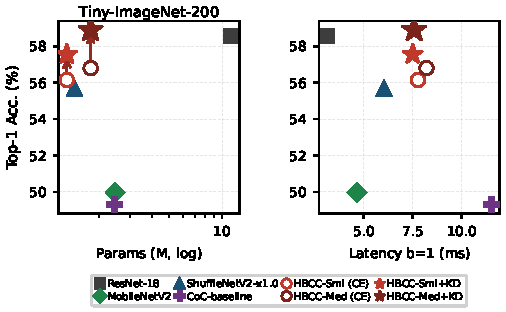
\includegraphics[width=\columnwidth]{pareto_tin}
  \caption{Pareto frontier on Tiny-ImageNet-200. Arrows: KD gains.
           HBCC-Medium+KD~($\bigstar$) surpasses ResNet-18 on both
           axes with 6.26$\times$ fewer parameters.}
  \label{fig:paretotin}
\end{figure}

\begin{figure}[ht!]
  \centering
  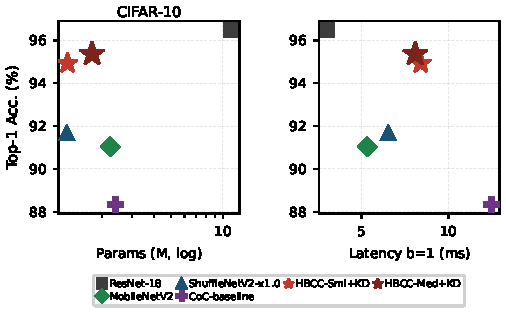
\includegraphics[width=\columnwidth]{pareto_cifar10}
  \caption{Pareto frontier on CIFAR-10. HBCC+KD occupies the
           Pareto-dominant region on both the parameter and latency
           axes relative to all lightweight baselines.}
  \label{fig:pareto10}
\end{figure}

\begin{figure}[ht!]
  \centering
  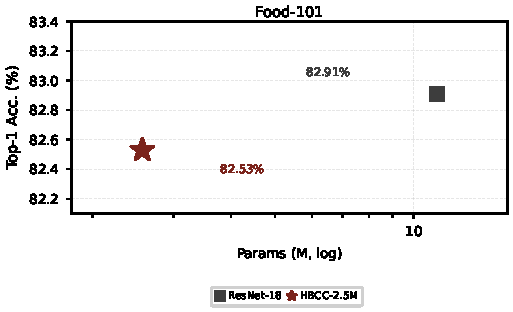
\includegraphics[width=\columnwidth]{pareto_food101}
  \caption{Parameter efficiency on Food-101 (parameter axis only;
           latency not profiled at $224\!\times\!224$).
           HBCC-2.5M~($\bigstar$) reaches 82.53\% with
           4.38$\times$ fewer parameters than ResNet-18.}
  \label{fig:paretofood}
\end{figure}

\subsubsection{Latency and Peak Memory Analysis}
\label{ssec:latency}

\noindent\textbf{Latency: Fewer MACs, Yet Slower.}
Although HBCC-Medium uses fewer MACs than ResNet-18 (138.9M
vs.\ 556.8M), its batch-1 latency is higher ($\approx\!8$\,ms
vs.\ $\approx\!3$\,ms) due to \textit{operator fragmentation}:
ResNet-18 runs $\approx\!94\%$ of CUDA time inside one optimized
kernel (\texttt{cudnn\_convolution}), while HBCC distributes it across
many small kernels ($1\!\times\!1$ convs, batch matmul, cosine
normalization, scatter/gather). HBCC nonetheless runs 30--35\%
faster than pure CoC (8\,ms vs.\ 11\,ms).

\noindent\textbf{Peak Memory: Scatter Buffers Dominate.}
HBCC-Medium reaches 481.6\,MB (47\% above ResNet-18's 326.7\,MB)
because scatter/gather aggregation holds a similarity tensor and a
feature sum per stage simultaneously; \texttt{stem\_stride=1} makes
these buffers $4\!\times$ larger than in the stride-2 CoC-baseline
(72.0\,MB). Reducing \texttt{stem\_stride} is the most direct lever.

\subsection{Discussion on Suitability and Application Scope}
\label{sec:discussion}

\textbf{Results scale with class-space complexity.}
On CIFAR-10 (10 classes), the 1.12\% gap reflects ResNet-18's strong
local inductive bias: local texture suffices and the gap is produced
by a model with $6\times$ more parameters --- acceptable under strict
resource constraints. On Tiny-ImageNet-200 (200 fine-grained classes),
the ranking reverses: HBCC-Medium+KD surpasses the teacher by 0.32\%
with $6.26\times$ fewer parameters, confirming that contextual
advantage grows with class-space complexity.

\textbf{Why knowledge distillation is particularly effective on
fine-grained benchmarks.}
Temperature-softened distributions ($T{=}4.0$) encode inter-class
relationships: semantically adjacent classes (e.g., dog breeds, or
tools of similar shape) receive non-negligible probability mass from
the teacher, providing richer supervision than one-hot labels. The
context clustering mechanism in Stages~3--4 aggregates global spatial
information through assignment and weighted summation --- a structure
better suited to absorbing inter-class relational signals than local
convolution, which processes patches independently and lacks a
mechanism to model global class similarity. This explains why KD
gains on Tiny-ImageNet-200 ($+$2.10\%/$+$1.41\%) are sufficient for
the student to surpass the teacher: the clustering architecture
exploits soft distributions more effectively than the convolutional
teacher architecture itself when the class space is large enough.

\textbf{Design implications from the local branch ablation.}
The gap between HBCC and CoC-baseline widens from $+$7.02\% on
CIFAR-10 to $+$9.60\% on Tiny-ImageNet-200, confirming that the value
of the local branch increases with classification complexity.
LBPConv at Stage~1 encodes parameter-free binary texture features;
DWConv at Stage~2 refines local shape information; together they
supply spatially local discriminative signals that pure global
clustering cannot learn from aggregation alone. This suggests a
general design principle: at high-resolution stages, low-parameter
local operators achieve a better information-to-cost ratio than
global clustering, and their complementary combination becomes more
critical as the number of classes grows.

\textbf{Food-101: scalable and balanced.}
At $224\!\times\!224$ with 101 classes, the gap narrows to 0.38\% top-1
with $4.38\times$ fewer parameters, demonstrating that the hybrid design
scales to standard-resolution inputs without sacrificing parameter
efficiency. Notably, HBCC's best checkpoint appeared at the final
training epoch, suggesting the 0.38\% gap is an upper bound on the
true architectural difference and may narrow further with a larger
training budget.

\textbf{When HBCC is the right choice.}
HBCC is most appropriate when: (i)~the class space is large
($\gtrsim\!100$ categories); (ii)~input resolution is sufficient to
avoid token degeneracy; and (iii)~the parameter budget is strictly
constrained. For few-class tasks without resource constraints, a
standard lightweight CNN remains more efficient. In practice, HBCC
targets fine-grained edge scenarios --- food identification, plant
disease classification, wildlife monitoring --- where contextual
aggregation and parameter efficiency provide the greatest benefit.

\textbf{Limitations and future directions.}
Operator fragmentation is the main practical challenge: HBCC runs
slower than ResNet-18 despite fewer MACs because the aggregation and
dispatch steps rely on multiple small GPU kernels that are not
individually optimized. Fused CUDA kernel implementations for these
steps could substantially reduce latency without any architectural
change. Peak memory is elevated by \texttt{stem\_stride=1}, which
retains $32\!\times\!32$ feature maps through Stage~1; adaptive
striding or similarity-tensor quantization are candidate mitigations.
Narrow margins on Tiny-ImageNet-200 (0.32\,pp) and Food-101 (0.38\,pp)
require confirmation across multiple independent seeds. Natural
extensions include object detection and semantic segmentation, where
global context aggregation may provide greater benefit than in image
classification.

% ============================================================
\section{Conclusion}
\label{sec:conclusion}

HBCC is a four-stage hybrid architecture that applies local processing
(LBPConv, DWConv) at high-resolution stages and pure Context Cluster
at lower resolutions, co-designed with \texttt{stem\_stride=1} and
stage-shrinking folds to prevent token degeneracy.
HBCC-Medium+KD achieves \textbf{95.36\%} on CIFAR-10 and
\textbf{58.90\%} on Tiny-ImageNet-200 --- surpassing the ResNet-18
teacher with $6.26\times$ fewer parameters; HBCC-2.5M achieves
\textbf{82.53\%} on Food-101 ($224\!\times\!224$) with $4.38\times$
fewer parameters than ResNet-18. Crucially, a 1.80M-parameter student
surpassing its 11.27M-parameter teacher on a 200-class benchmark
confirms that context clustering exploits the teacher's soft
distributions more effectively than the convolutional teacher
architecture itself when the class space is sufficiently complex.

Results confirm that HBCC's contextual advantage scales with
classification complexity --- marginal on CIFAR-10, decisive on
Tiny-ImageNet-200, balanced on Food-101 --- making it most valuable
for fine-grained recognition under tight parameter budgets.
Three design principles are established: (i)~stage-specific operator
selection matched to feature-map resolution optimizes the
information-to-cost ratio; (ii)~progressive fold shrinking prevents
token degeneracy without adding parameters; (iii)~low-parameter local
branches supply spatially local discriminative signals that global
clustering lacks, with their value increasing as the number of classes
grows.

Primary limitations to be addressed: narrow margins
(Tiny-ImageNet-200: 0.32\,pp; Food-101: 0.38\,pp) require multi-seed
confirmation; operator fragmentation keeps latency and memory above
convolutional baselines with comparable MACs; Food-101 results reflect
the combined effect of architecture and training recipe rather than
architecture alone. Future work will focus on fused CUDA kernel
implementations to close the latency gap, adaptive striding to reduce
peak memory, and extending evaluation to object detection and semantic
segmentation.

% ============================================================
\bibliographystyle{IEEEtran}
\bibliography{references}

\end{document}